%!TeX program = xelatex
%Do not change
\documentclass[12pt, oneside]{article}
\usepackage{amssymb,amsmath}
\usepackage[margin=1in]{geometry}
\usepackage{textpos}
\usepackage{float}
\usepackage{booktabs}
%\usepackage{color}
\usepackage{graphicx}
\usepackage[inter-unit-product =\cdot]{siunitx}
\let\DeclareUSUnit\DeclareSIUnit
\let\US\SI
\DeclareUSUnit\inch{in}
\DeclareUSUnit\foot{ft}
\DeclareUSUnit\mile{mi}
\DeclareUSUnit\foot{ft}
\DeclareUSUnit\slug{slug}
\DeclareUSUnit\pound{lb}
\DeclareUSUnit\psi{psi}
\DeclareUSUnit\Msi{Msi}
\DeclareUSUnit\ksi{ksi}

\usepackage{tikz}
\usetikzlibrary{positioning}
%\usepackage{tikz-3dplot}
\usepackage{pgfopts}
%\usepackage{wasysym}
\usepackage{stanli}

% You may add the packages you need here
\begin{document}

%TODO change numbers in problems
\begin{textblock*}{4cm}(-1.7cm,-2.3cm)
\noindent {\scriptsize AE333 Fall 2020}
\end{textblock*}

%Do not modify other than putting your name where stated
\begin{textblock*}{8cm}(12.5cm,-1cm)
\noindent {Name: }
\end{textblock*}
%Do not modify other than typing your acknowledgement where stated
\begin{textblock*}{13.5cm}(-1.7cm,-1.8cm)
%\noindent \textit{\footnotesize Acknowledgement: Your acknowledgement for collaboration and other sources goes here. }
\end{textblock*}

\vspace{1cm}

%Do not modify other than typing the homework number after #
\begin{center}
\textbf{\Large Homework 10}
\end{center}

\begin{enumerate}
	\item %4-92
		Determine the maximum normal stress developed in the bar when it is subjected to a tension of $P = 	\US{4 }{kip} $
		\begin{figure}[H]
			\centering
			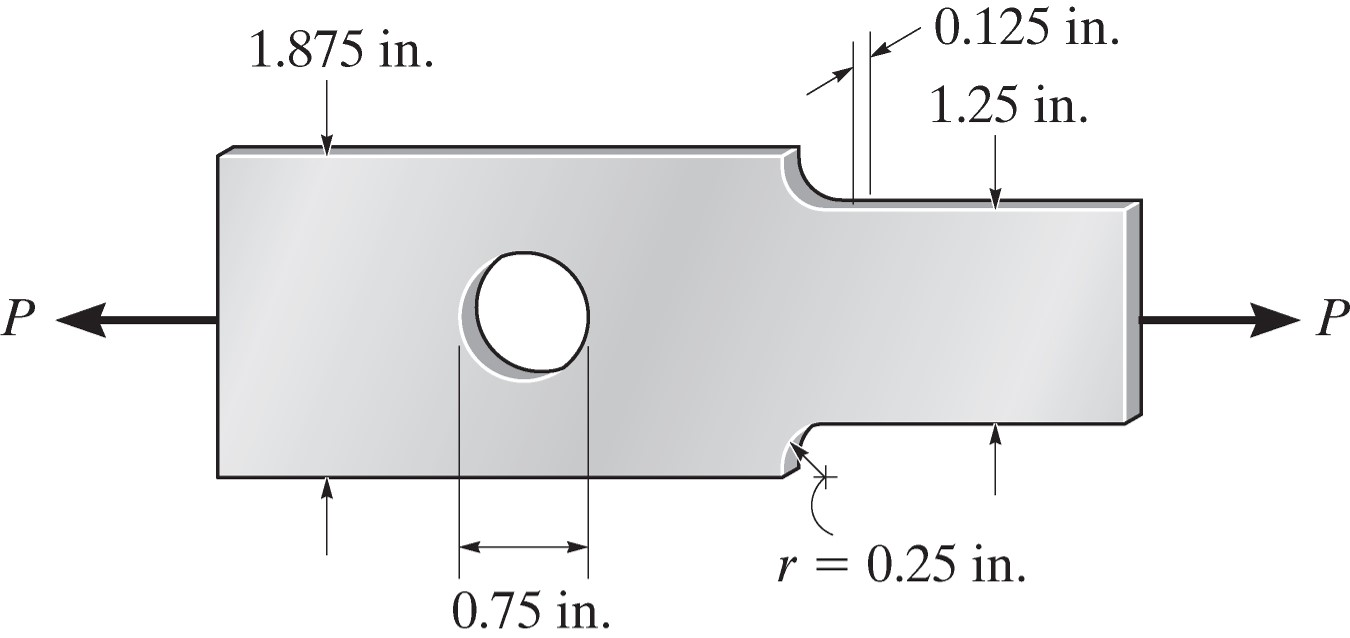
\includegraphics[width=0.8\linewidth]{4-92}
		\end{figure}
			\textbf{Solution:}
			\begin{itemize}
				\item To find the maximum normal stress we need to find the maximum stress from the hole and the fillet and determine which is greater.
				\item We start by finding the stress concentration factor for the hole. We have $2r/w = 0.4$ which gives $K = 2.2$. Using $\sigma_{avg} = \frac{N}{(w-2r)t}$ we find $\sigma_{max} = 	\US{62.6}{ksi} $
				\item For the fillet we find $w/h = 1.5$ and $r/h = 0.2$ which gives $K = 1.7$. Using $\sigma_{avg} = \frac{N}{ht}$ we find $\sigma_{max} = 	\US{43.5 }{ksi} $
				\item We find that the maximum normal stress is caused by the hole and has a value of $\sigma_{max} = 	\US{62.6}{ksi} $
			\end{itemize}

	\item %4-90
		The A-36 steel plate has a thickness of $ 	\SI{12 }{mm}  $.
		If $\sigma_{allow} = 	\SI{135 }{MPa} $, determine the maximum axial load, $P$ that it can support.
		\begin{figure}[H]
			\centering
			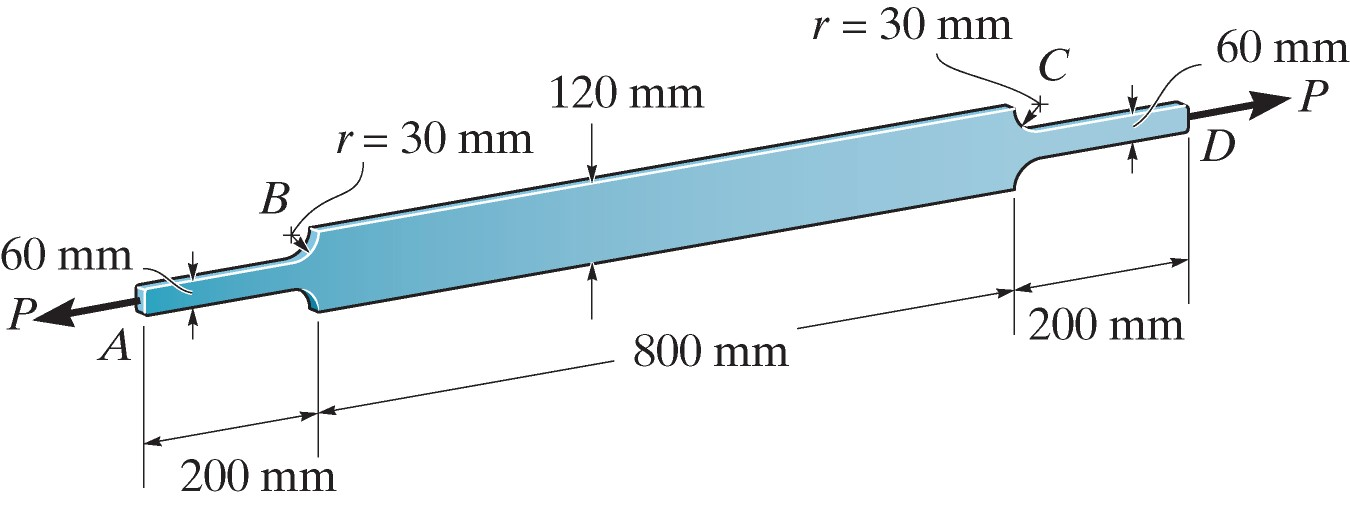
\includegraphics[width=0.6\linewidth]{4-90}
		\end{figure}
			\textbf{Solution:}
			\begin{itemize}
				\item In this case we use $\sigma_{allow} = K \sigma_{avg}$ to find the maximum $P$ that we can support
				\item For the fillet geometry shown we have $w/h = 2$ and $r/h = 0.5$ which gives $K = 1.4$
				\item We can now solve $ 	\SI{135 }{MPa} = \frac{1.4 P}{60 \cdot 12}  $ for $P$ to find $P = 	\SI{69.4 }{kN} $
			\end{itemize}

	\item %5-124
		The shaft is fixed to the wall at $A$ and is subjected to the torques shown.
		Find the maximum shear stress in the shaft.
		A fillet weld having a radius of $ 	\SI{2.75 }{mm}  $ is used to connect the shafts at $B$
		\begin{figure}[H]
			\centering
			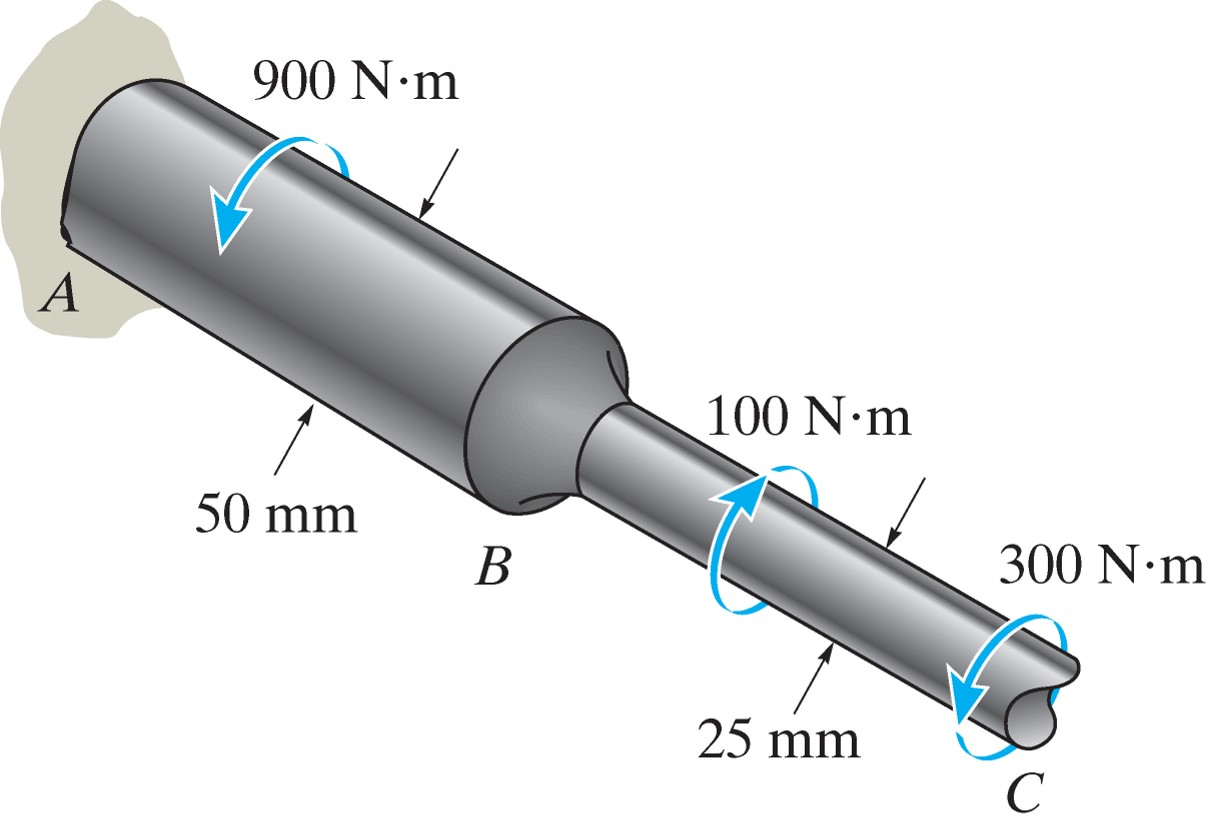
\includegraphics[width=0.6\linewidth]{5-124}
		\end{figure}
			\textbf{Solution:}
			\begin{itemize}
				\item From statics we find internal torques of $ 	\SI{1100}{N.m}  $ between the wall and the first torque, $ 	\SI{200 }{N.m}  $ between the first and second torques and $ 	\SI{300}{N.m}  $ between the second and third torques. There is a fillet between the first and second torques to increase the maximum stress.
				\item We calculate shear stress from torsional load in the usual way with $\tau = \frac{Tc}{J}$, which gives $\tau_1 = 	\SI{44.8 }{MPa} $, $\tau_2 = 	\SI{65.2 }{MPa} $ and $\tau_3 = 	\SI{97.8 }{MPa} $
				\item Applying the stress concentration factor to the region with the fillet ($\tau_2$) we find $D/d = 2.0$ and $r/d = 0.22$ we find $K \approx 1.21$ which gives $\tau_2 = 	\SI{78.9 }{MPa} $
				\item This is still less than $\tau_3$, which means maximum shear stress in the shaft is $\tau_3 = 	\SI{97.8 }{MPa} $
			\end{itemize}

	\item %6-155
		If the radius of each notch on the plate is $ 	\SI{10 }{mm}  $ find the largest moment $M$ that can be applied.
		The maximum allowable bending stress is $\sigma_{allow} = 	\SI{190}{MPa} $
		\begin{figure}[H]
			\centering
			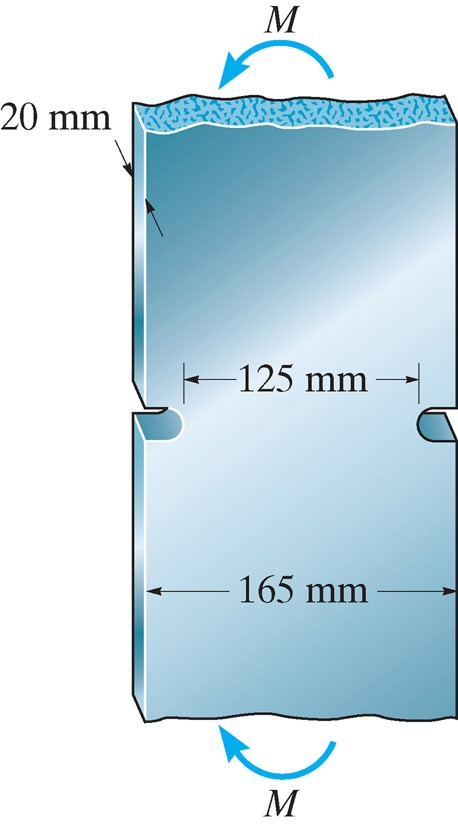
\includegraphics[width=0.3\linewidth]{6-155}
		\end{figure}
			\textbf{Solution:}
			\begin{itemize}
				\item We can use the bending stress formula $ 	\SI{190 }{MPa} = \frac{KMy}{I}  $ to solve for $M$.
				\item We can find $K$ from the chart with $r/h = .08$ and $b/r = 2.0$, which gives $K = 2.1$.
				\item With $y = 	\SI{62.5 }{mm}$ and $I = 	\SI{3.26e6}{mm^4} $ we find $M = 	\SI{4.71}{kN.m} $
			\end{itemize}

	\item %13-14
		The W8 x 67 flange 2014-T6 aluminum column can be assumed to be fixed at its base and pinned at its top.
		Find the largest axial force, $P$, that can be applied without causing buckling.
		\begin{figure}[H]
			\centering
			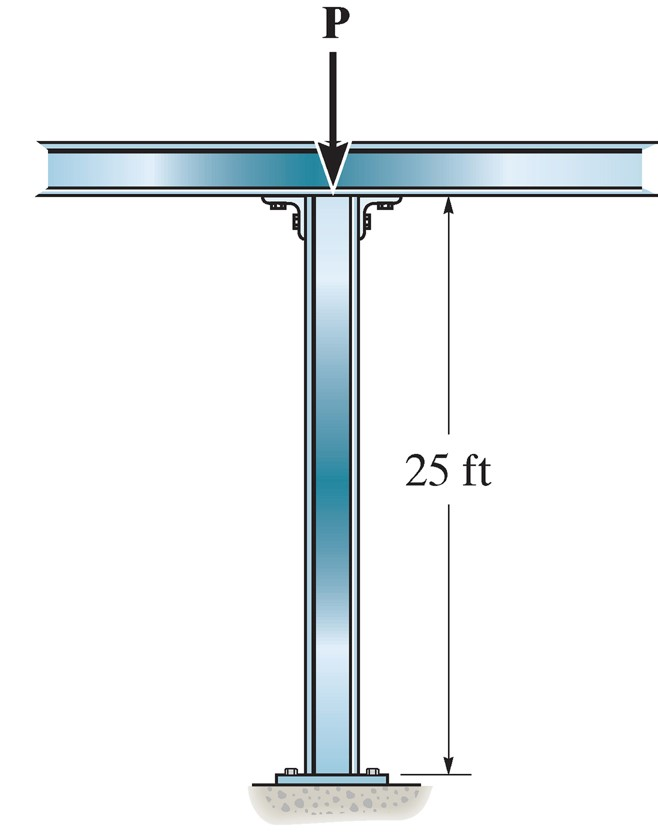
\includegraphics[width=0.6\linewidth]{13-14}
			\caption{13-14}%
			\label{fig:13-14}
		\end{figure}
			\textbf{Solution:}
			\begin{itemize}
				\item The buckling formula in terms of load is $P_{cr} = \frac{\pi^2 EI}{(KL)^2}$
				\item For the given column we have $E = 	\US{10.6}{Msi} $ and $I = 	\US{272}{in^4} $ about the $x-x$ axis and $I = 	\US{88.6}{in^4} $ about the $y-y$ axis. We can clearly see that the buckling load will be lower about the $y-y$ axis, so that will be our limiting case.
				\item For a fixed-pinned beam, the length factor $K = 0.7$
				\item We can substitute these values to find $P_{cr} = 	\US{210}{klb} $ 
			\end{itemize}

	\item %13-15
		Solve the previous problem assuming that it is fixed at its base and free at its top
			\textbf{Solution:}
			\begin{itemize}
				\item For a fixed-free column we change the length factor to $K = 2.0$ which gives a critical load of $P_{cr} = 	\US{25.6}{klb} $
			\end{itemize}

	\item
		Repeat the previous problems assuming that it is fixed at both the base and top.
		Which of these cases is the best for buckling, which is the worst?
			\textbf{Solution:}
			\begin{itemize}
				\item A fixed-fixed column has a length factor of $K = 0.5$ which gives $P_{cr} = 	\US{412}{klb} $
				\item It is not surprising that the fixed-fixed beam is the best and the fixed-free is the worst in buckling, but it may be somewhat surprising how strong the differences are.
				\item The fixed-fixed column can support almost double the load of the fixed-pinned column without buckling, while supporting almost 20 times the load of the fixed-free column.
			\end{itemize}

\end{enumerate}
\end{document}
